\tikzset{every picture/.style={line width=0.75pt}} %set default line width to 0.75pt        

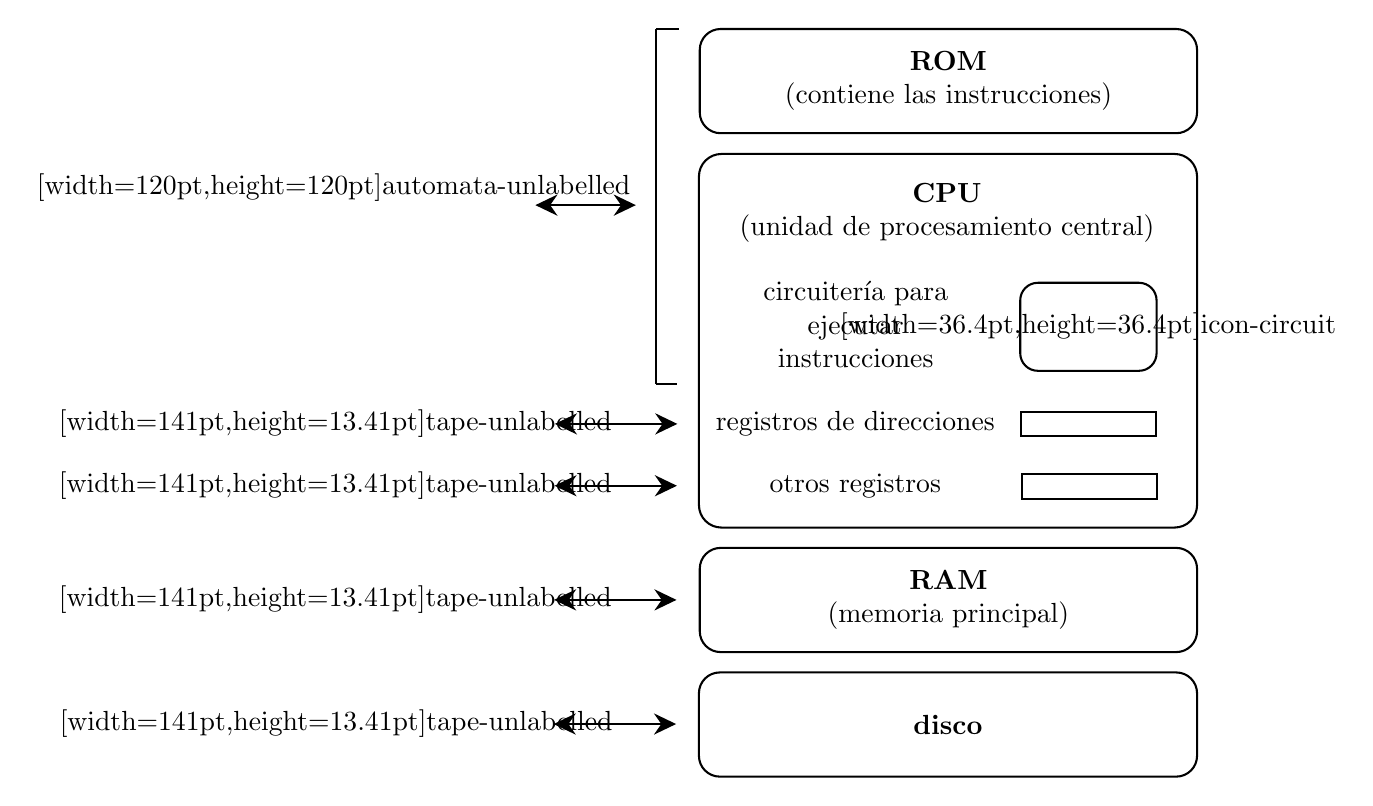
\begin{tikzpicture}[x=0.75pt,y=0.75pt,yscale=-1,xscale=1]
%uncomment if require: \path (0,629); %set diagram left start at 0, and has height of 629

%Image [id:dp5052356785139098] 
\draw (144,146.6) node  {\includesvg[width=120pt,height=120pt]{automata-unlabelled}};
%Rounded Rect [id:dp16008108582529212] 
\draw   (320.4,80.04) .. controls (320.4,74.5) and (324.9,70) .. (330.44,70) -- (549.96,70) .. controls (555.5,70) and (560,74.5) .. (560,80.04) -- (560,110.16) .. controls (560,115.7) and (555.5,120.2) .. (549.96,120.2) -- (330.44,120.2) .. controls (324.9,120.2) and (320.4,115.7) .. (320.4,110.16) -- cycle ;
%Rounded Rect [id:dp8550659349752405] 
\draw   (320,141.07) .. controls (320,135.06) and (324.86,130.2) .. (330.87,130.2) -- (549.13,130.2) .. controls (555.14,130.2) and (560,135.06) .. (560,141.07) -- (560,299.33) .. controls (560,305.34) and (555.14,310.2) .. (549.13,310.2) -- (330.87,310.2) .. controls (324.86,310.2) and (320,305.34) .. (320,299.33) -- cycle ;
%Rounded Rect [id:dp3980421004805672] 
\draw   (320.4,330.04) .. controls (320.4,324.5) and (324.9,320) .. (330.44,320) -- (549.96,320) .. controls (555.5,320) and (560,324.5) .. (560,330.04) -- (560,360.16) .. controls (560,365.7) and (555.5,370.2) .. (549.96,370.2) -- (330.44,370.2) .. controls (324.9,370.2) and (320.4,365.7) .. (320.4,360.16) -- cycle ;
%Rounded Rect [id:dp8207352186926025] 
\draw   (320,390.04) .. controls (320,384.5) and (324.5,380) .. (330.04,380) -- (549.96,380) .. controls (555.5,380) and (560,384.5) .. (560,390.04) -- (560,420.16) .. controls (560,425.7) and (555.5,430.2) .. (549.96,430.2) -- (330.04,430.2) .. controls (324.5,430.2) and (320,425.7) .. (320,420.16) -- cycle ;
%Image [id:dp4653438326616097] 
\draw (144.8,260.3) node  {\includesvg[width=141pt,height=13.41pt]{tape-unlabelled}};
%Shape: Rectangle [id:dp231624424338565] 
\draw   (475.2,254.6) -- (540.2,254.6) -- (540.2,266.26) -- (475.2,266.26) -- cycle ;
%Shape: Rectangle [id:dp8216158761938366] 
\draw   (475.6,284.6) -- (540.6,284.6) -- (540.6,296.26) -- (475.6,296.26) -- cycle ;
%Straight Lines [id:da7645694678182564] 
\draw    (253.6,260.26) -- (306.6,260.26) ;
\draw [shift={(309.6,260.26)}, rotate = 180] [fill={rgb, 255:red, 0; green, 0; blue, 0 }  ][line width=0.08]  [draw opacity=0] (10.72,-5.15) -- (0,0) -- (10.72,5.15) -- (7.12,0) -- cycle    ;
\draw [shift={(250.6,260.26)}, rotate = 0] [fill={rgb, 255:red, 0; green, 0; blue, 0 }  ][line width=0.08]  [draw opacity=0] (10.72,-5.15) -- (0,0) -- (10.72,5.15) -- (7.12,0) -- cycle    ;
%Straight Lines [id:da441650131991439] 
\draw    (253.4,290.06) -- (306.4,290.06) ;
\draw [shift={(309.4,290.06)}, rotate = 180] [fill={rgb, 255:red, 0; green, 0; blue, 0 }  ][line width=0.08]  [draw opacity=0] (10.72,-5.15) -- (0,0) -- (10.72,5.15) -- (7.12,0) -- cycle    ;
\draw [shift={(250.4,290.06)}, rotate = 0] [fill={rgb, 255:red, 0; green, 0; blue, 0 }  ][line width=0.08]  [draw opacity=0] (10.72,-5.15) -- (0,0) -- (10.72,5.15) -- (7.12,0) -- cycle    ;
%Straight Lines [id:da026287841550500568] 
\draw    (253.2,345.06) -- (306.2,345.06) ;
\draw [shift={(309.2,345.06)}, rotate = 180] [fill={rgb, 255:red, 0; green, 0; blue, 0 }  ][line width=0.08]  [draw opacity=0] (10.72,-5.15) -- (0,0) -- (10.72,5.15) -- (7.12,0) -- cycle    ;
\draw [shift={(250.2,345.06)}, rotate = 0] [fill={rgb, 255:red, 0; green, 0; blue, 0 }  ][line width=0.08]  [draw opacity=0] (10.72,-5.15) -- (0,0) -- (10.72,5.15) -- (7.12,0) -- cycle    ;
%Straight Lines [id:da39421236199134] 
\draw    (253,404.86) -- (306,404.86) ;
\draw [shift={(309,404.86)}, rotate = 180] [fill={rgb, 255:red, 0; green, 0; blue, 0 }  ][line width=0.08]  [draw opacity=0] (10.72,-5.15) -- (0,0) -- (10.72,5.15) -- (7.12,0) -- cycle    ;
\draw [shift={(250,404.86)}, rotate = 0] [fill={rgb, 255:red, 0; green, 0; blue, 0 }  ][line width=0.08]  [draw opacity=0] (10.72,-5.15) -- (0,0) -- (10.72,5.15) -- (7.12,0) -- cycle    ;
%Straight Lines [id:da9170493361927601] 
\draw    (299.4,240.86) -- (309.4,240.86) ;
%Straight Lines [id:da15556503654230558] 
\draw    (299.4,69.86) -- (310.4,69.86) ;
%Straight Lines [id:da21370062507016763] 
\draw    (299.4,69.86) -- (299.4,240.86) ;
%Straight Lines [id:da659991079227169] 
\draw    (244.2,154.86) -- (286.6,154.86) ;
\draw [shift={(289.6,154.86)}, rotate = 180] [fill={rgb, 255:red, 0; green, 0; blue, 0 }  ][line width=0.08]  [draw opacity=0] (10.72,-5.15) -- (0,0) -- (10.72,5.15) -- (7.12,0) -- cycle    ;
\draw [shift={(241.2,154.86)}, rotate = 0] [fill={rgb, 255:red, 0; green, 0; blue, 0 }  ][line width=0.08]  [draw opacity=0] (10.72,-5.15) -- (0,0) -- (10.72,5.15) -- (7.12,0) -- cycle    ;
%Image [id:dp8580690474170394] 
\draw (507.49,213.48) node  {\includesvg[width=36.4pt,height=36.4pt]{icon-circuit}};
%Rounded Rect [id:dp036199891504040904] 
\draw   (474.8,200.75) .. controls (474.8,196.07) and (478.6,192.27) .. (483.28,192.27) -- (532.01,192.27) .. controls (536.69,192.27) and (540.49,196.07) .. (540.49,200.75) -- (540.49,226.2) .. controls (540.49,230.88) and (536.69,234.68) .. (532.01,234.68) -- (483.28,234.68) .. controls (478.6,234.68) and (474.8,230.88) .. (474.8,226.2) -- cycle ;
%Image [id:dp8048596501026082] 
\draw (144.8,289.9) node  {\includesvg[width=141pt,height=13.41pt]{tape-unlabelled}};
%Image [id:dp1557490659088474] 
\draw (144.8,344.9) node  {\includesvg[width=141pt,height=13.41pt]{tape-unlabelled}};
%Image [id:dp8233409398311418] 
\draw (145.2,404.7) node  {\includesvg[width=141pt,height=13.41pt]{tape-unlabelled}};

% Text Node
\draw (440.2,95.1) node   [align=left] {\begin{minipage}[lt]{162.7pt}\setlength\topsep{0pt}
\begin{center}
\textbf{ROM}\\(contiene las instrucciones)
\end{center}

\end{minipage}};
% Text Node
\draw (439.53,158.55) node   [align=left] {\begin{minipage}[lt]{162.7pt}\setlength\topsep{0pt}
\begin{center}
\textbf{CPU}\\(unidad de procesamiento central)
\end{center}

\end{minipage}};
% Text Node
\draw (395.5,212.33) node   [align=left] {\begin{minipage}[lt]{88.17pt}\setlength\topsep{0pt}
\begin{center}
circuitería para ejecutar instrucciones
\end{center}

\end{minipage}};
% Text Node
\draw (395.33,260.17) node   [align=left] {\begin{minipage}[lt]{102pt}\setlength\topsep{0pt}
\begin{center}
registros de direcciones
\end{center}

\end{minipage}};
% Text Node
\draw (395.33,290.17) node   [align=left] {\begin{minipage}[lt]{102pt}\setlength\topsep{0pt}
\begin{center}
otros registros
\end{center}

\end{minipage}};
% Text Node
\draw (440.2,345.1) node   [align=left] {\begin{minipage}[lt]{162.7pt}\setlength\topsep{0pt}
\begin{center}
\textbf{RAM}\\(memoria principal)
\end{center}

\end{minipage}};
% Text Node
\draw (440,405.1) node   [align=left] {\begin{minipage}[lt]{162.7pt}\setlength\topsep{0pt}
\begin{center}
\textbf{disco}
\end{center}

\end{minipage}};


\end{tikzpicture}